\documentclass[11pt]{homework}
\usepackage[margin=1in]{geometry}
\usepackage{float}
\fancyheadoffset{0cm}

\newcommand{\hwname}{Luis Pimentel ~~~~~~~~~~~~~~ Jackson Crandell}
\newcommand{\professor}{Professor Evangelos Theodorou}
\newcommand{\hwemail}{lpimentel3@gatech.edu ~~~ jackcrandell@gatech.edu}
\newcommand{\hwtype}{Homework}
\newcommand{\hwnum}{3}
\newcommand{\hwclass}{AE 4803 Robotics and Autonomy}
\newcommand{\hwdate}{November 25, 2020}

\renewcommand{\vec}[1]{\ensuremath{\boldsymbol{#1}}}
\addtolength{\jot}{0.5em}
\allowdisplaybreaks

\usepackage[colorlinks=false]{hyperref}
\usepackage[ruled,vlined]{algorithm2e}

\usepackage{ dsfont }

\begin{document}
\maketitle

%%%%%%%%%%%%%%%%%%%%%%%%%%%%%%%%%%%%%%%%%%%%%%%%%%%%%%%%%%%%%%%%%%%%%%%%%%%%%%%%%%%%%%% Part 1 
\renewcommand{\questiontype}{Problem}
\question

	We formulate our experiment with the following scalar system:
	\begin{align*}
		& A=[0.4] \\
		& B=[0.9] \\
		& Q=[0.01] \\
		& R=[0.001]
	\end{align*}

	MATLAB's \vec{dlqr} function computes the optimal gain K = 0.3964. \\

	We formulate the following Reinforcement Learning optimization problem and solving using gradient ascent with Finite Differencing gradient estimation: 
	
	\begin{align*}
		& \underset{\theta}{\text{maximize}} \hspace{0.35cm} \mathbb{E}\Big[R(\vec{\tau}) \Big] \\
		& R(\vec{\tau}) = \sum_{t=0}^{N} r(\vec{x}_{t},\vec{u}_{t},t) \\
		& r(\vec{x}_{t},\vec{u}_{t},t) = -\vec{x}^T \vec{Q}\vec{x} - \vec{u}^{T}\vec{R}\vec{u} \\
		& \vec{u} = -\vec{\theta}\vec{x}
	\end{align*}
	
	This results in an optimal $\vec{\theta}^{\star}$ = 0.3990. Our convergence criterion fulfills that the gradient is sufficiently small for some $\epsilon$ or that our Reward begins to decrease after increasing for a certain number of times.  
	
	\begin{figure}[H]
		\centering
		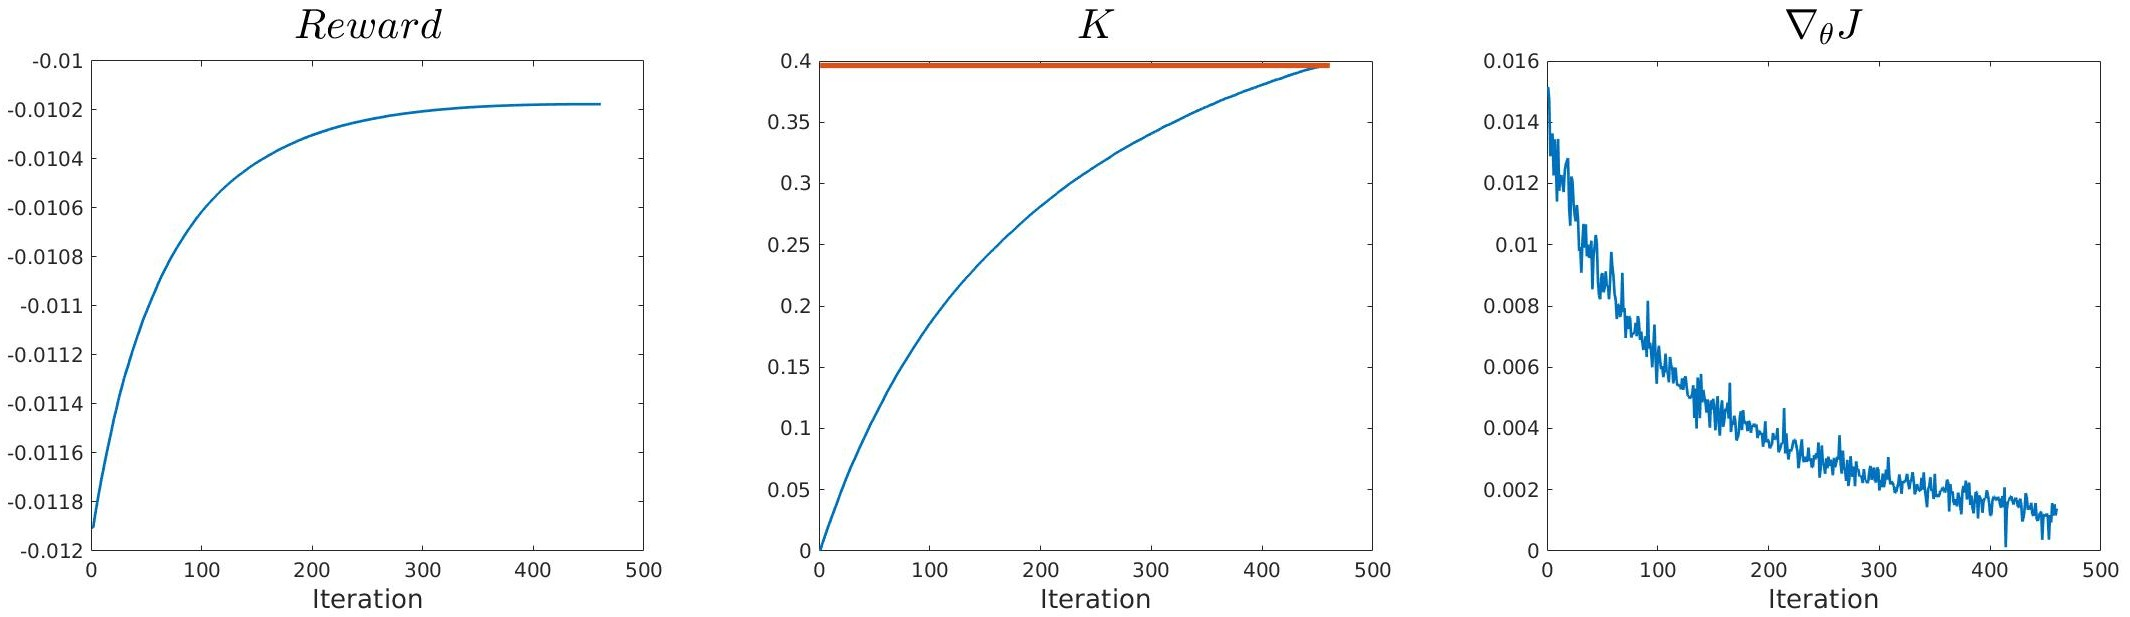
\includegraphics[scale=0.23]{finite_differencing_results}
		\caption{Results using Finite Differencing policy gradient estimation.}
		\label{}
	\end{figure}


%%%%%%%%%%%%%%%%%%%%%%%%%%%%%%%%%%%%%%%%%%%%%%%%%%%%%%%%%%%%%%%%%%%%%%%%%%%%%%%%%%%%%%% Part 3 
\renewcommand{\questiontype}{Problem}
\question
\begin{arabicparts}
%\setcounter{questionCounter}{2}

\questionpart

	For the derivation of the REINFORCE Gradient we begin with the following cost function: 

		\begin{align*}
			& J(\vec{\theta}) = \int p(\vec{\tau})R(\vec{\tau}) \,d\vec{\tau} 
		\end{align*}
		
	A trajectory can be expressed as $\vec{\tau} = (\vec{x_{0}}, \vec{u_{0}},\dots,\vec{x_{N-1}}, \vec{u_{N-1}}, \vec{x_{N})}$ with states $\vec{x} \in \mathds{R}^{\ell}$ and controls $\vec{u} \in \mathds{R}^{p}$ over the time horizon T = Ndt. R(\vec{\tau}) is the accumalated cost over a trajectory and $p(\vec{\tau})$ represents the path probability of the trajectory, which using Bayesian and Markov properties can be expressed as: 
	
		\begin{align*}
			& p(\vec{\tau}) = p(\vec{x}_0)\prod_{i=0}^{N-1} p(\vec{x}_{i+1}|\vec{x}_i,\vec{u}_i)p(\vec{u}_{i}|\vec{x}_{i};\vec{\theta}) \\
			& R(\vec{\tau}) = \sum_{t=0}^{N-1} r(\vec{x}_{t},\vec{u}_{t},t) 
		\end{align*}
	
	The $p(\vec{u}_{i}|\vec{x}_{i};\vec{\theta})$ term in path probability represents the parametrized policy where $\vec{\theta} \in  \mathds{R}^{n}$. We begin our derivation by the gradient of the cost function with respect to $\vec{\theta}$, $\nabla_{\vec{\theta}}J(\vec{\theta})$. 
		
		 \begin{align*}
			& \nabla_{\vec{\theta}}J(\vec{\theta}) = \nabla_{\vec{\theta}}\Bigg( \int p(\vec{\tau})R(\vec{\tau}) \,d\vec{\tau} \Bigg) \\
			& \int \nabla_{\vec{\theta}}p(\vec{\tau})R(\vec{\tau}) \,d\vec{\tau} \\
		\end{align*}
	
	We use the following log property:
		\begin{align*}
			& \nabla_{\vec{\theta}} log(p(\vec{\tau})) = \frac{1}{p(\vec{\tau})}\nabla_{\vec{\theta}} p(\vec{\tau}) \\
			& \nabla_{\vec{\theta}} p(\vec{\tau}) = p(\vec{\tau})\nabla_{\vec{\theta}} log(p(\vec{\tau}))
		\end{align*}

		To make the substitution and rewrite the following as an expectation:
		\begin{align*}
			& \int p(\vec{\tau})\nabla_{\vec{\theta}} log(p(\vec{\tau}))R(\vec{\tau}) \,d\vec{\tau} \\
			& E_{p(\vec{\tau})}\Bigg[\nabla_{\vec{\theta}} log(p(\vec{\tau}))R(\vec{\tau})\Bigg]
		\end{align*}

	We start by calculating $\nabla_{\vec{\theta}} log(p(\vec{\tau}))$ 

		\begin{align*}
			& \nabla_{\vec{\theta}} log(p(\vec{\tau})) = \nabla_{\vec{\theta}}log\Bigg( p(\vec{x}_0)\prod_{i=0}^{N-1} p(\vec{x}_{i+1}|\vec{x}_i,\vec{u}_i)p(\vec{u}_{i}|\vec{x}_{i};\vec{\theta}) \Bigg) \\
			& = \nabla_{\vec{\theta}}log(p(\vec{x}_0)) + \nabla_{\vec{\theta}}log\Bigg( \prod_{i=0}^{N-1} p(\vec{x}_{i+1}|\vec{x}_i,\vec{u}_i)\Bigg) +  \nabla_{\vec{\theta}}log\Bigg( \prod_{i=0}^{N-1}p(\vec{u}_{i}|\vec{x}_{i};\vec{\theta})\Bigg) \\
			& = \nabla_{\vec{\theta}}log(p(\vec{x}_0)) + \nabla_{\vec{\theta}}\sum_{i=0}^{N-1} log(p(\vec{x}_{i+1}|\vec{x}_i,\vec{u}_i)) +  \nabla_{\vec{\theta}}\sum_{i=0}^{N-1}log(p(\vec{u}_{i}|\vec{x}_{i};\vec{\theta})) \\
			& = \sum_{i=0}^{N-1}\nabla_{\vec{\theta}}log(p(\vec{u}_{i}|\vec{x}_{i};\vec{\theta}))
		\end{align*}

	From this we rewrite our policy gradient as
		\begin{align*}
			& \nabla_{\vec{\theta}}J(\vec{\theta}) = E_{p(\vec{\tau})}\Bigg[\sum_{i=0}^{N-1}\nabla_{\vec{\theta}}log(p(\vec{u}_{i}|\vec{x}_{i};\vec{\theta}))R(\vec{\tau})\Bigg]
		\end{align*}

	We can further simplify this by calculating $p(\vec{u}_{i}|\vec{x}_{i};\vec{\theta})$ given the parametrized policy with Gaussian noise $\epsilon \sim \mathcal{N}(0,\vec{I})$:
		\begin{align*}
			& u(\vec{x}, \vec{\theta},t_{k}) = \vec{\Phi}(\vec{x})\vec{\theta} + \vec{B}(\vec{x})\epsilon(t_{k})
		\end{align*}

	We start by expressing $p(\vec{u}_{i}|\vec{x}_{i};\vec{\theta})$ as the multi-variate Gaussian Distribution: 
		\begin{align*}
			& p(\vec{u}_{i}|\vec{x}_{i};\vec{\theta}) = \frac{1}{(2\pi)^{m/2}| \vec{B}(\vec{x})\vec{B}(\vec{x})^{T}|^{1/2}}exp\Bigg( -\frac{1}{2}(\vec{u} - \vec{\Phi}(\vec{x})\vec{\theta})^{T}\Big(\vec{B}(\vec{x})\vec{B}(\vec{x})^T\Big)^{-1}(\vec{u}-\vec{\Phi}(\vec{x})\vec{\theta})  \Bigg)\\
		\end{align*}
	
	We then express $log(p(\vec{u}_{i}|\vec{x}_{i};\vec{\theta}))$ as: 
	
	\begin{align*}
		&  log(p(\vec{u}_{i}|\vec{x}_{i};\vec{\theta})) = log\Bigg(  \frac{1}{(2\pi)^{m/2}| \vec{B}\vec{B}^{T}|^{1/2}}exp\Big( -\frac{1}{2}(\vec{u} - \vec{\Phi}\vec{\theta})^{T}\Big(\vec{B}\vec{B}^T\Big)^{-1}(\vec{u}-\vec{\Phi}\vec{\theta})  \Big)    \Bigg) \\
		& = log\Bigg( \frac{1}{(2\pi)^{m/2}| \vec{B}\vec{B}^{T}|^{1/2}} \Bigg) + log\Bigg( exp\Big( -\frac{1}{2}(\vec{u} - \vec{\Phi}\vec{\theta})^{T}\Big(\vec{B}\vec{B}^T\Big)^{-1}(\vec{u}-\vec{\Phi}\vec{\theta})  \Big)  \Bigg)\\
		& = -log\Big( (2\pi)^{m/2}\vec{B}\vec{B}^{T}|^{1/2} \Big) - \frac{1}{2}(\vec{u} - \vec{\Phi}\vec{\theta})^{T}\Big(\vec{B}\vec{B}^T\Big)^{-1}(\vec{u}-\vec{\Phi}\vec{\theta}) \\
		& = -log\Big( (2\pi)^{m/2}\vec{B}\vec{B}^{T}|^{1/2} \Big) - \frac{1}{2}(\vec{u}^{T} -\vec{\theta}^{T} \vec{\Phi}^{T})\Big(\vec{B}\vec{B}^T\Big)^{-1}(\vec{u}-\vec{\Phi}\vec{\theta}) \\
		& = -log\Big( (2\pi)^{m/2}\vec{B}\vec{B}^{T}|^{1/2} \Big) + \Bigg(-\frac{1}{2}\vec{u}^{T}\Big(\vec{B}\vec{B}^T\Big)^{-1}  + \frac{1}{2}\vec{\theta}^{T}\vec{\Phi}^{T}\Big(\vec{B}\vec{B}^T\Big)^{-1}\Bigg)(\vec{u}-\vec{\Phi}\vec{\theta}) \\
		& = -log\Big( (2\pi)^{m/2}\vec{B}\vec{B}^{T}|^{1/2} \Big)  -\frac{1}{2}\vec{u}^{T}\Big(\vec{B}\vec{B}^T\Big)^{-1}\vec{u}	+ \frac{1}{2}\vec{\theta}^{T}\vec{\Phi}^{T}\Big(\vec{B}\vec{B}^T\Big)^{-1}\vec{u} + \frac{1}{2}\vec{u}^{T}\Big(\vec{B}\vec{B}^T\Big)^{-1}\vec{\Phi}\vec{\theta} \\
		& - \frac{1}{2}\vec{\theta}^{T}\vec{\Phi}^{T}\Big(\vec{B}\vec{B}^T\Big)^{-1}\vec{\Phi}\vec{\theta} \\
		& = -log\Big( (2\pi)^{m/2}\vec{B}\vec{B}^{T}|^{1/2} \Big)  -\frac{1}{2}\vec{u}^{T}\Big(\vec{B}\vec{B}^T\Big)^{-1}\vec{u} + \vec{\theta}^{T}\vec{\Phi}^{T}\Big(\vec{B}\vec{B}^T\Big)^{-1}\vec{u} - \frac{1}{2}\vec{\theta}^{T}\vec{\Phi}^{T}\Big(\vec{B}\vec{B}^T\Big)^{-1}\vec{\Phi}\vec{\theta} \\
	\end{align*}
	
	We then compute the gradient of this expression with respect to $\vec{\theta}$ and substitute our parametrized policy $\vec{u} = \vec{\Phi}\vec{\theta} + \vec{B}\epsilon_{k}$:
	
	\begin{align*}
		& \nabla_{\vec{\theta}}log(p(\vec{u}_{i}|\vec{x}_{i};\vec{\theta})) = \vec{\Phi}^{T}\Big(\vec{B}\vec{B}^T\Big)^{-1}\vec{u} - \vec{\Phi}^{T}\Big(\vec{B}\vec{B}^T\Big)^{-1}\vec{\Phi}\vec{\theta} \\
		& = \vec{\Phi}^{T}\Big(\vec{B}\vec{B}^T\Big)^{-1}\Bigg( \vec{\Phi}\vec{\theta} + \vec{B}\epsilon_{k}  \Bigg) - \vec{\Phi}^{T}\Big(\vec{B}\vec{B}^T\Big)^{-1}\vec{\Phi}\vec{\theta} \\
		& = \vec{\Phi}^{T}\Big(\vec{B}\vec{B}^T\Big)^{-1}\vec{\Phi}\vec{\theta} + \vec{\Phi}^{T}\Big(\vec{B}\vec{B}^T\Big)^{-1}\vec{B}\epsilon_{k} - \vec{\Phi}^{T}\Big(\vec{B}\vec{B}^T\Big)^{-1}\vec{\Phi}\vec{\theta} \\
		& = \vec{\Phi}^{T}\Big(\vec{B}\vec{B}^T\Big)^{-1}\vec{B}\epsilon_{k}
	\end{align*}
	
	Now given that $\nabla_{\vec{\theta}}log(p(\vec{u}_{i}|\vec{x}_{i};\vec{\theta})) = \vec{\Phi}^{T}\Big(\vec{B}\vec{B}^T\Big)^{-1}\vec{B}\epsilon_{k}$ we turn can rewrite our gradient policy: 
	\begin{align*}
		& \nabla_{\vec{\theta}}J(\vec{\theta}) = E_{p(\vec{\tau})}\Bigg[\sum_{i=0}^{N-1}\nabla_{\vec{\theta}}log(p(\vec{u}_{i}|\vec{x}_{i};\vec{\theta}))R(\vec{\tau})\Bigg] \\
		& = E_{p(\vec{\tau})}\Bigg[R(\vec{\tau})\sum_{i=0}^{N-1} \vec{\Phi}^{T}\Big(\vec{B}\vec{B}^T\Big)^{-1}\vec{B}\epsilon_{k}\Bigg]
	\end{align*}
	
	If we paramtrize the policy such that $\Phi = \vec{B}$ then the final form of the REINFORCE Gradient can be written as: 
	\begin{align*}
		& \nabla_{\vec{\theta}}J(\vec{\theta}) = E_{p(\vec{\tau})}\Bigg[R(\vec{\tau})\sum_{i=0}^{N-1} \vec{B}^{T}\Big(\vec{B}\vec{B}^T\Big)^{-1}\vec{B}\epsilon_{i}\Bigg]
	\end{align*}
	For this implementation our policy controller takes the following form where $\Phi = \vec{B} = \vec{x}_{i}$
	\begin{align*}
		& \vec{u}_i = \vec{\vec{\theta}}\vec{x}_{i} + \epsilon_{i}\vec{x}_{i} 
	\end{align*}
	Therefore the gradient takes the following form: 
	\begin{align*}
		& \nabla_{\vec{\theta}}J(\vec{\theta}) = E_{p(\vec{\tau})}\Bigg[R(\vec{\tau})\sum_{k=0}^{N-1} \vec{x}_{i}^{T}\Big(\vec{x}_{i}\vec{x}_{i}^T\Big)^{-1}\vec{x}_{i}\epsilon_{k}\Bigg] \\
		& = E_{p(\vec{\tau})}\Bigg[R(\vec{\tau})\sum_{i=0}^{N-1}\epsilon_{i}\Bigg] \\
		& = \frac{1}{M}\sum_{m=0}^{M}\Bigg(\Big(\sum_{i=0}^{N-1}\epsilon_{m,i}\Big) \Big(\sum_{i=0}^{N-1} r(\vec{x}_{m,i},\vec{u}_{m,i},i)\Big) \Bigg)
	\end{align*}

	\questionpart
	
	For our experiment we formulate the same system as in Problem 1 which results in the same optimal LQR gain K = 0.3964.
	
	We formulate the same Reinforcement Learning optimization problem as before and solve it using gradient ascent and REINFORCE policy gradient estimation. 
	
	This results in an optimal $\vec{\theta}^{\star}$ = 0.3968. Our convergence criterion fulfills that the gradient is sufficiently small for some $\epsilon$ or that our Reward begins to decrease after increasing for a certain number of times.
	
	\begin{figure}[H]
		\centering
		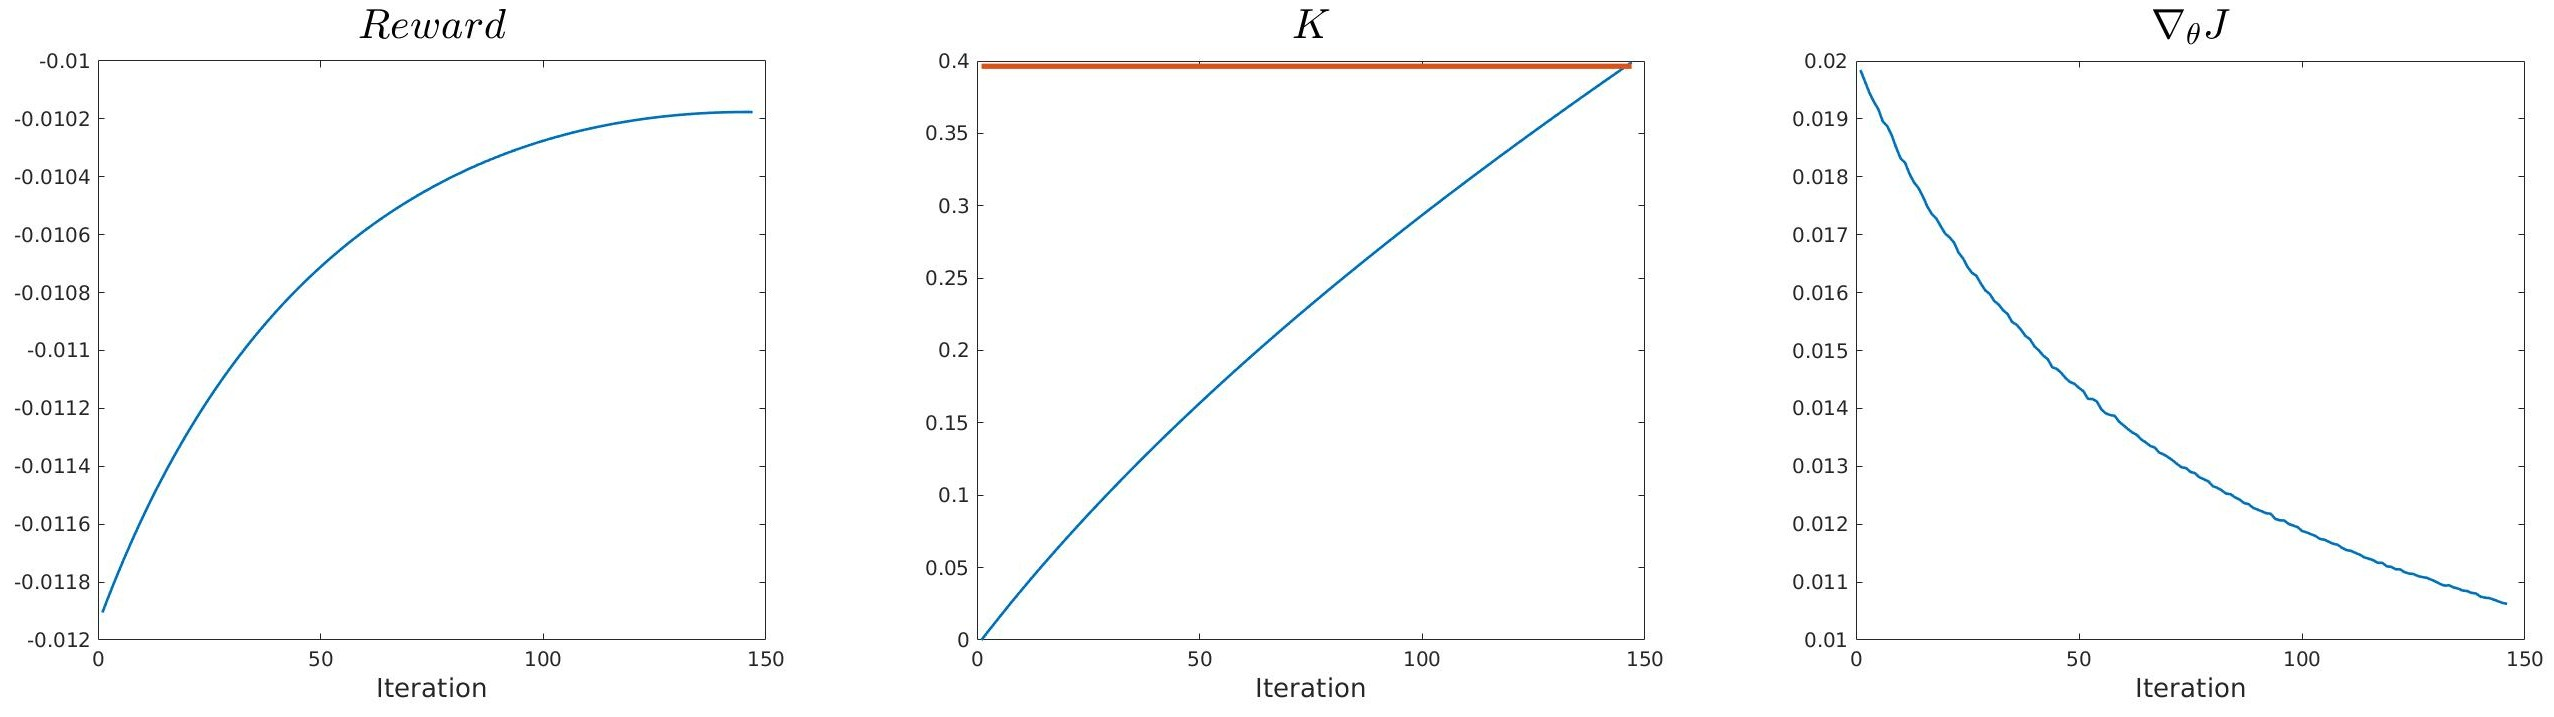
\includegraphics[scale=0.19]{reinforce_results.jpg}
		\caption{Results using REINFORCE policy gradient estimation.}
		\label{}
	\end{figure}
	
\end{arabicparts}

	







\end{document}
